\documentclass[man, 12pt]{apa7} % 'man' for manuscript, 12pt font size

\usepackage[american]{babel} % American English
\usepackage{csquotes} % Recommended with biblatex


% Bibliography setup for APA style
\usepackage[style=apa, sortcites=true, sorting=nyt, backend=biber]{biblatex}
\addbibresource{mahbod.bib} % Your .bib file
\DeclareLanguageMapping{american}{american-apa}

% Additional useful packages
\usepackage{graphicx} % For including graphics
\usepackage{booktabs} % For professional quality tables
\usepackage{amsmath} % Enhanced math support
\usepackage{amsfonts} % Additional math fonts
\usepackage{amssymb} % Extended symbol collection
\usepackage{hyperref} % For hyperlinks in the document

% Margins and spacing adjustments if needed
\usepackage{geometry}
\geometry{
    left=1in,
    right=1in,
    top=1in,
    bottom=1in
}
\usepackage{setspace}
\doublespacing % or \onehalfspacing

% Title, authors, and affiliations
\title{TBD}
\shorttitle{TBD}
\author{Mahbod Mehrvarz, Jeffrey N. Rouder}
\affiliation{{University of California, Irvine}}
\leftheader{Weiss}

% Author note
\authornote{
   \addORCIDlink{TBD}{0000-0000-0000-0000}
   Version 2, Nov, 2023.
  
   Author Contributions: JNR MM  
  
   JNR was supported by NSF 2126976.
}

% Abstract and Keywords
\abstract{
    Abstract Here
}
\keywords{TK, TK}


\begin{document}

\maketitle



In the modern landscape, researchers study cognitive abilities like perception, language, problem-solving, and memory through the lens of information processing. The main focus is on understanding how our minds represent, manage, combine, store, recall, and assess information from our surroundings. A prevalent method to identifying such abilities is using the \textit{experimental} design, which is characterized by having multiple conditions that can be contrasted to control for factors not under study. For example, to measure \textbf{cognitive control}--the ability to inhibit proponent responses--tasks such as Stroop employ congruent and incongruent conditions. The difference in response times between the two conditions is utilized to construct a measure for cognitive control. The said contrast and the manipulation through experimental conditions provide much-desired theoretically validated and interpretable measures for the cognitive ability under study. 

A critical inquiry within this context involves investigating the variations in cognitive abilities across different individuals. Specifically, is there a discernible and consistent pattern of variation between individuals? Over the past two decades, considerable focus has been placed on finding such a pattern in cognitive control. Cognitive control and related concepts of inhibition, executive function, and self-regulation have been central in theories of attention, development, aging, performance, and psychopathology. Because of this centrality, the structure and correlates of cognitive control have been studied repeatedly with individual differences using experimental tasks. However, finding a pattern of variation has proven difficult. 

This difficulty perhaps reflects a statistical concern that goes by the moniker of \textbf{reliability crisis}. That is, measures of cognitive abilities obtained through the experimental design often lack sufficient reliability to perform latent variable modeling. Three characteristics observed in recent inquiries have exemplified this concern. First, several tasks that purportedly measure the same construct do not correlate well. For example, the correlation between flanker and Stroop effects in large studies is often near .1 and rarely greater than .25. \parencite{Enkavi.etal.2019, Rey-Mermet.etal.2019, Rouder.etal.2023}. Second, factor-model analyses have not proved replicable or robust.  The evidence comes from \Textcite{Karr.etal.2018}, who showed that when bootstrapped simulated data were submitted to confirmatory-factor-model analysis, the best-fitting model from the original set was rarely recovered. Finally, it has been observed that individual differences in experiments have low reliability \parencite{Hedge.etal.2018, Draheim.etal.2019}.  How people differ in an experiment does not predict with high precision how they will differ again.


How bad is this problem?  We will explore the scope of the problem in depth, but the following brief example may serve as motivation.  Consider an experiment with six tasks.  Each task is comprised of two conditions---a congruent and an incongruent condition---with the latter requiring more cognitive control than the former.  In this setup, trials are nested in conditions; for instance, a participant might perform 100 trials in each condition for each task. The focal point of interest here is the participant's score, calculated as the difference in average performance between the incongruent and congruent conditions, and the critical question is how these scores covary across the tasks. With six tasks at hand, we encounter 15 distinct inter-task correlations. For simplicity, let's posit that each task correlates with every other task at a true value of $\rho=.5$. This uniform correlation is depicted in the first column of Figure \ref{fig:prob_setup}A, under the label \textit{Truth}, as a single point at 0.5. We simulated data from this setup with 200 participants using realistic values for true performance (details to be discussed later). The next column, labeled \textit{Usual}, is the ordinary Pearson sample correlation estimate from participant scores.  Note that these sample correlations miss dramatically the true ones, for they are all too small.  Indeed, this attenuation of correlation is a well-known phenomena that occurs when scores are particularly prone to measurement error \parencite{Spearman.1987} and occurs often experimental contexts \parencite{Hedge.etal.2018,Enkavi.etal.2019,Rouder.Haaf.2019}.  A challenging aspect of this attenuation is that it is \textbf{asymptotic}.  As the number of individuals in the experiment is increased, attenuation does not decrease.  Rather, the analyst becomes increasing confidence in a badly attenuated value.

One long-standing strategy to mitigate attenuation is to calculate how much attenuation may be present and adjust accordingly, a process called \textbf{disattenuation}. Spearman proposed a simple formula \footnote{Spearman's correction for attenuation, expressed as $r^*_{xy} = \frac{r_{xy}}{\sqrt{r_{xx}\cdot r_{yy}}}$, recalibrates the observed correlations $r_{xy}$ between two variables by accounting for measurement error, assuming the errors are independent and uncorrelated, with $r_{xx}$ and $r_{yy}$ representing the respective test-retest reliabilities of the two variables.}, now known as Spearman's correction for disattenuation \parencite{Spearman.1987}. The third column in Figure \ref{fig:prob_setup}A presents the 15 correlations post-application of Spearman's correction. As advertised, these are disattenuated and center around the true value.  Yet, there are highly variable.  Context for this degree of variability comes from the size of the simulated experiment, which is comprised of 240,000 observations (calculated from 200 individuals each participating in 100 trials across two conditions in six tasks).  One might assume that accurately estimating 15 correlation coefficients from such a large data set would be straightforward. However, the reality is strikingly different: the disattenuated correlations range widely from .2 to .8, deviating on average by .18. The extent of uncertainty in such a large data set is highly disconcerting. This inability to localize correlations in reasonable cognitive-control settings serves as the problem for this report.



Why is localizing these correlations important?  There are two reasons.  First, the correlation (or covariation) among tasks serves as a critical target in doumenting and communicating the relations among tasks.  Second, this covariation is almost always further decomposed using latent variable models such as factor analysis and structural equation modeling.  The effectiveness of these latent variable decompositions hinges critically on the precision with which these correlations may be pinpointed. In cases where correlations are imprecisely determined or dramatically attenuated, the resulting latent structure may be only weakly identifiable, casting doubt on the validity of any inferences drawn from it \parencite{Karr.etal.2018}.

Several recent approaches have been proposed to address the issue of poor localization. For instance, \textcite{Draheim.etal.2019} recommends adopting measures that do not depend on contrasting conditions, such as those that differentiate between congruent and incongruent task components. Another strategy other researchers recommended involves using gamification \parencite[]{Deveau.etal.2015, Kucina.etal.2023, Wells.etal.2021}. In gamification, cognitive control experiments are integrated into an engaging computer video game format, complete with stimulating music and a competitive points system. The goal is to elicit more pronounced participant responses and encourage longer engagement in gamified cognitive control tasks.
Meanwhile, our research \parencite[]{Rouder.Haaf.2019}, along with that of others \parencite{Haines.etal.2023, Matzke.etal.2017}, has advocated an alternative solution, that is, the implementation of hierarchical models. These models are designed to simultaneously address variability both in individual trials and across participants.  The hope is that by using these models, researchers can better localize correlations.

Yet, from our experience, the anticipated benefits of hierarchical models in localizing correlations have not fully materialized. \textcite{Rouder.etal.2023} used a simulation approach to assess whether hierarchical models could indeed localize correlations in reasonable designs with realistic effects. The final column of Figure \ref{fig:prob_setup}A shows correlations from a hierarchical model to be presented subsequently. Rouder et al. identified three key advantages of the hierarchical approach, two of which are evident in Figure \ref{fig:prob_setup}A.  First, hierarchical-model analysis typically leads to less attenuation compared to the usual approach. Second, it achieves more precise localization than Spearman's disattenuation method, with overall Root Mean Square Error (\textbf{RMSE}) improvements of about $20\%$. Third, and importantly, unlike the other two approaches, hierarchical models offer a realistic assessment of uncertainty in correlations. The last benefit is illustrated in Figure \ref{fig:prob_setup}B. The orange histogram is the posterior distribution of one of the correlations. The orange dashed lines indicate the $95\%$ credible interval.  This interval is large, spanning from .27 to .76 in value.  Its size shows the high degree of uncertainty, which in turn, reflects a high degree of variability in performance from trial to trial.  In contrast, the usual estimate is shows as a green point.  The segments show the  $95\%$ confidence interval.  The relatively narrow confidence interval reflects the large number of participants without consideration of trial-to-trial variability. The usual correlation is greatly attenuated (true value is denoted with the purple line at .5) indicating that this high level of confidence is, in fact, misplaced. 

Despite these three benefits, the main problem remains---the improvement in localization is not as substantial as one might hope. In experiments of reasonable size, RMSEs remained high, often around .15, suggesting that even with a large data set of 240,000 observations, discerning whether a correlation was .3 or .7 remains elusive.  Localizing correlations with hierarchical models is challenging even in large data sets.


\subsection{Constrained and Unconstrained Hierarchical Models}

One strategy for increasing the precision of estimates is to use simpler and more constrained models.  For example, the slope of a regression term will increase in precision if higher order terms are left from the model.  We call this a pay-to-play strategy.  We propose using constrained hierarchical models that are designed to increase the precision of estimating covariation.  The approach, of course, is not cost free---the constraints we impose have to be realistic and warranted.  Potential constraints we explore are a positive manifold across covariation and a low-dimensional factor structure across tasks.

The pay-to-play strategy is best explained with a more formal specification of the models.  Consider a battery of cognitive control tasks where $I$ individuals each perform $J$ tasks. Each task is comprised of a congruent and an incongruent condition, and each individual performs $L$ trials in each condition. Let $i=1,\ldots,I$ index individuals, $j=1,\ldots,J$ index tasks, $k=1,2$ index conditions, and $\ell=1,\ldots,L$ denote replicate trials. Let $Y_{ijk\ell}$ denote the performance on the trial, for example the response time.  We place a linear model on it:
\begin{equation} \label{eq:RT_surface}
Y_{ijk\ell} = \alpha_{ij} + x_k\theta_{ij} + \epsilon_{ijk\ell}.
\end{equation}

In this model, $x_k$ is the contrast code for the two conditions, set at $\frac{-1}{2}$ and $\frac{1}{2}$ for congruent and incongruent conditions, respectively. The parameter $\alpha_{ij}$ is the true overall speed of the $i$th participant on the $j$th task. The parameter $\theta_{ij}$ is the true difference between incongruent and congruent conditions for the $j$th task---it is the $i$th participant's true effect on the $j$th task and is the focal point of analysis.  The error term is $\epsilon_{ijk\ell} \sim \mbox{Normal}(0,\tau^2)$, with $\tau^2$ describing the variability of trial noise \footnote{This model presumes a balanced design; each condition is spread equally across all trials and participants. This balance enforces uniformity in data collection, resulting in fewer potential biases. The assumption of equal variance ($\tau^2$) across trials and conditions, often referred to as homoscedasticity, implies that the variability in response times is consistent throughout the experiment across participants and conditions. In this paper, for the sake of simplicity, we adopt the premise that response time variability is consistent across tasks. Otherwise, the model would necessitate distinct variance terms for each task, denoted as $\tau_j^2$.}. 


The critical component of this model is the set of true effects ($\theta_{ij}$). Conventionally, individuals are treated as exchangeable. Tasks, in contrast, are not, and the relations among the tasks are of great interest. To capture this state of affairs, let $(\theta_{i1},\ldots,\theta_{iJ})$ be a column vector true effects for the $i$th participant.  This column vector may be modeled as multivariate normal:

\begin{equation} \label{eq:true_effect_vec}
\begin{bmatrix}
\theta_{i1}\\ \vdots\\ \theta_{iJ}
\end{bmatrix} \sim \mbox{Normal}_J\left(
\begin{bmatrix}
\mu_1\\ \vdots\\ \mu_J
\end{bmatrix},
\begin{bmatrix}
\sigma_{11}&\ldots&\sigma_{1J}\\
\vdots &\ddots&\vdots\\
\sigma_{1J}&\ldots&\sigma_{JJ}
\end{bmatrix}
\right).
\end{equation}

Alternatively, this can be expressed more succinctly as follows:

\begin{equation} \label{eq:true_effect_mat}
\boldsymbol{\theta}_i \sim \mbox{N}_J(\boldsymbol{\mu},\boldsymbol{\Sigma}),
\end{equation}

Equation \ref{eq:true_effect_mat} describes an unconstrained model where $\boldsymbol{\Sigma}$ can take on any valid covariance matrix. 
The absence of constraints allows $\boldsymbol{\Sigma}$ to encompass any conceivable relationship among tasks. Consider the constraint from a one-factor model.  


Because there is no constraint on $\bfSigma$, it describes any set of relations among the tasks.  Constraint may be added by placing equality constraints across the elements of $\bfSigma$.  Consider the constraint from a one-factor model.  Figure X shows three equivalent representations of the one-factor constraint.  The first one is graphical, and there is a common factor, denoted "C" for *control* influencing the effects in all tasks.  The second representation is mathematical, it describes the constraint where off diagonal elements enter in ratio to the common factor.  The third representation is a graphical version of the covariance matrix.  Here, we see multiplicative pattern, for example, if Task 4 correlates highly with Task 5 and Task 6, then Task 5 and Task 6 must correlate highly as well. 

To see the constraint as parameter reduction, consider again that six tasks.  The unconstrained version has 21 free parameters (6 diagonal elements and 15 off-diagonal elements).  The one-factor constrained version has 12 free parameters, which is a bit more than half the free number of parameters.  @Bollen.1989 introduces latent variables models in this manner---each may be considered a constraint on a covariance matrix.

The hierarchical models in this report are the combination of (\ref{eq.base}) and (\ref{eq.theta}) along with constraints on $\bfSigma$ to be discussed subsequently.  These models are analyzed in the Bayesian framework because of computational tractability.  We leverage recent advances by [citations] in Bayesian analysis offactor models, and we implement our solutions in JAGS, a popular, general-purpose package for Bayesian analysis (all code is available at the github archive associated with this paper).  In contrast, we do not know how to analyze hierarchical factor models in the frequentist context.  To get an idea of the difficulty, consider that the observable in the hierarchical case are individual trial data rather than blah blah.


In the Bayesian framework, priors are placed on all parameters.  Our approach here is to use weakly informed subjective priors.  For example, the prior on overall true speed, $\alpha_{ij}$ is a normal with a mean of .8s and a standard deviation of 1s.  This specification is quite reasonable for cognitive control tasks like the Stroop or flanker where RTs are typically under a second.  Likewise, priors of $\sigma^2$ are broad with much mass between .01 and 1 (sec$^2$), which corresponds to broad prior on standard deviation of trial-to-trial noise with much mass between 100 ms and 1 sec.  Likewise, priors on $\mu$ in (\ref{eq.theta}) reflect the expected range of effects, where are between 0 and 150ms. [footnote, formal specification of priors]  The critical prior specifications are for $\bfSigma$, and we defend our choices subsequently.


## The Inverse-Wishart Unconstrained Model

The unconstrained model we use comes from @Haaf.Rouder.2017 and @Rouder.etal.inpress.  Here, an inverse Wishart prior is placed on $\bfSigma$: $\bfSigma \sim \mbox{Inv. Wishart}(m,\bfS)$, where $m$ and $bfS$ serve as prior settings on the shape and scale of the inverse Wishart that need to be made *a priori*.  The shape parameter is uninformative when set to the size of $\bfSigma$ which is $J$, or the number of tasks (Mahbod, check).  The scale parameter is a bit trickier.  A lack of *a prior* preference for negative or positive correlations comes when $\bfS=b^2\times\bfI$ where $\bfI$ is the diagonal matrix (of size $J$) and $b^2$ is an expected variance.  This expectation is made with reference to analysis of existing data sets as discussed subsequently.

JEFF Paragraph here about LKJ












% References
\printbibliography


\begin{figure}[htbp]
    \centering  % Centers the figure
    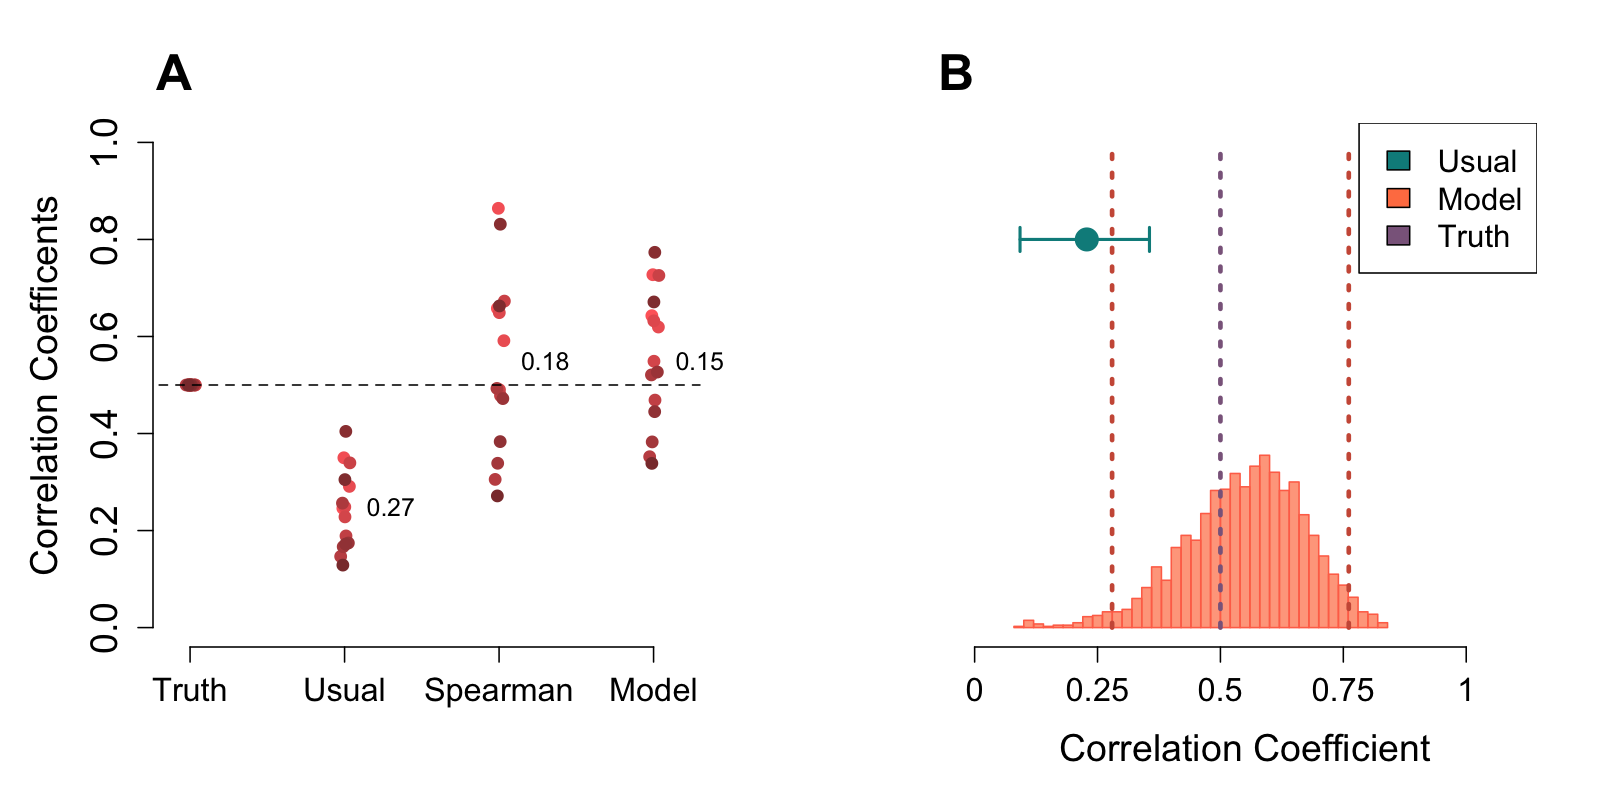
\includegraphics[width=\linewidth, height=1\linewidth, keepaspectratio]{_figs/prob_setupAll.png}
    \caption{A. A single run through a simulation where all correlations are .5 (Truth).  Shows are the usual Pearson sample correlations, the Spearman disattenuation correlations, and hierarchical model estimates.  The values next to the spread of points show the RMSEs in estimation.  B. A comparison of the usual Pearson sample correlation and the hierarchical model analysis.  The green point shows the usual estimate along with 95\% confidence intervals.  The orange distribution shows the posterior of the same blah blah the narrow ness misses the true value bluh bluh}  % Replace 'TK' with your actual caption.
    \label{fig:prob_setup}
\end{figure}

\begin{figure}[htbp]
    \centering  % Centers the figure
    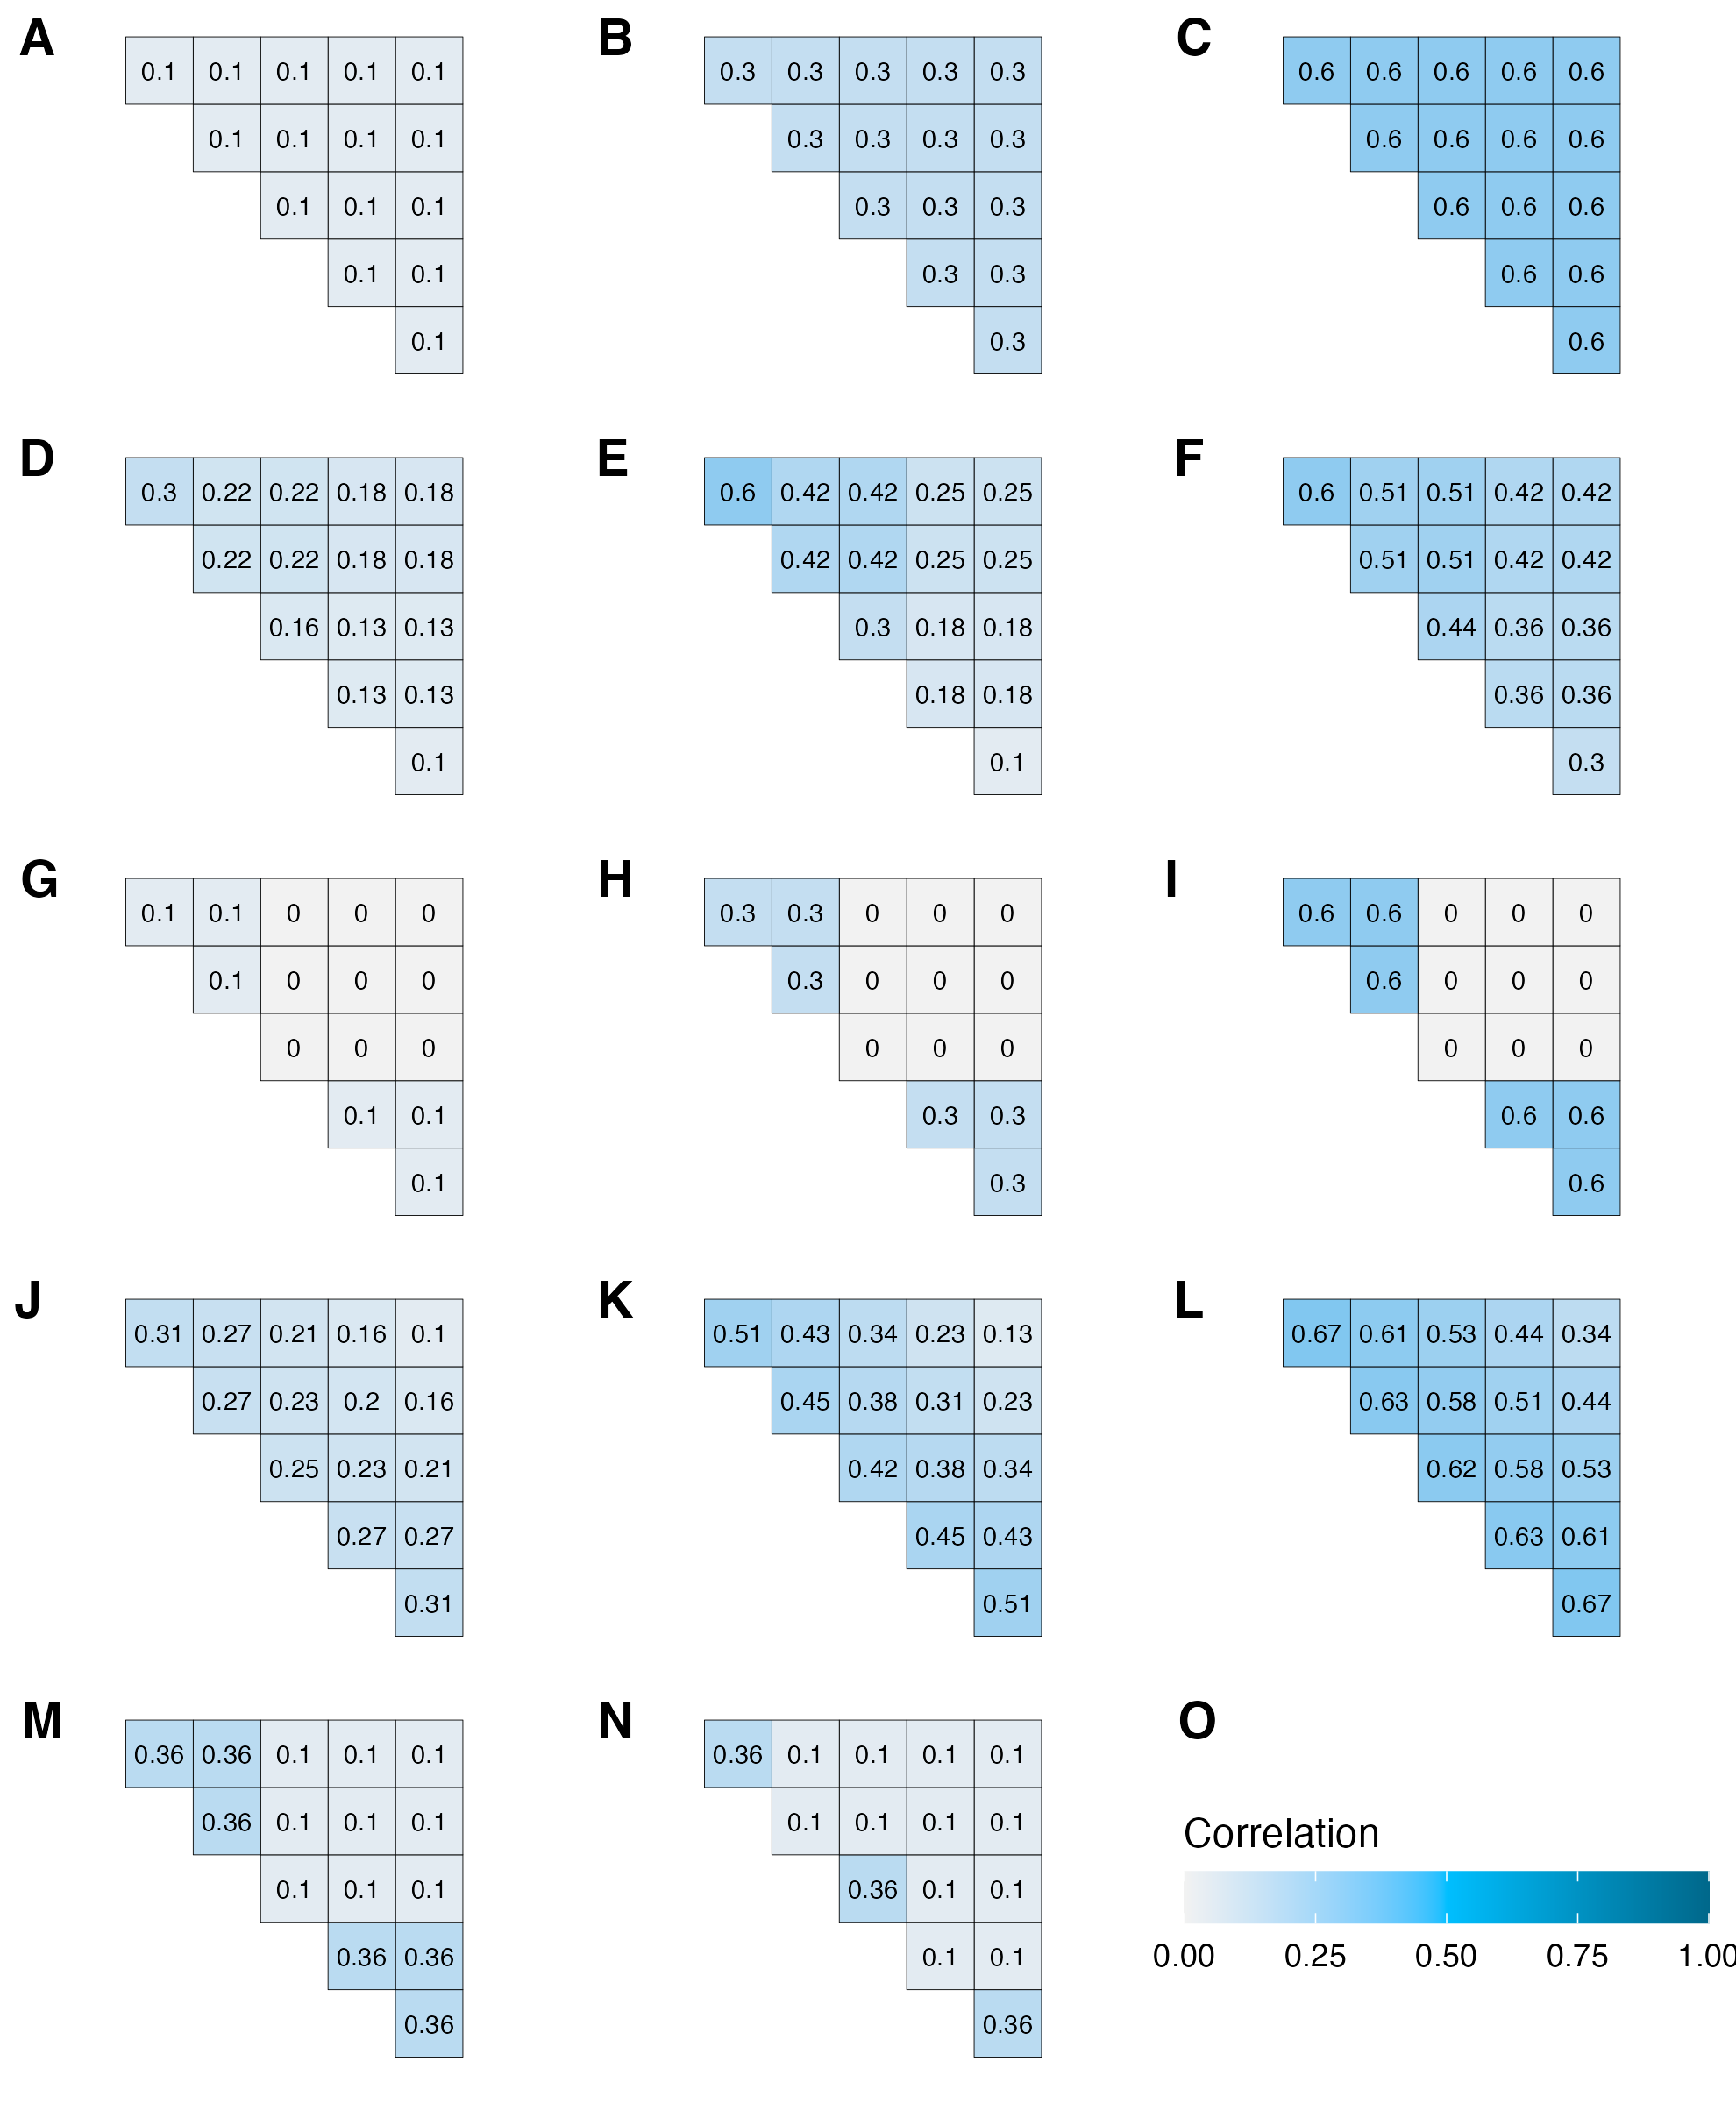
\includegraphics[width=\linewidth, height=1.1\linewidth, keepaspectratio]{_figs/true_cors.png}
    \caption{TK}  % Replace 'TK' with your actual caption.
    \label{fig:true_cors}
\end{figure}


\begin{figure}[htbp]
    \centering  % Centers the figure
    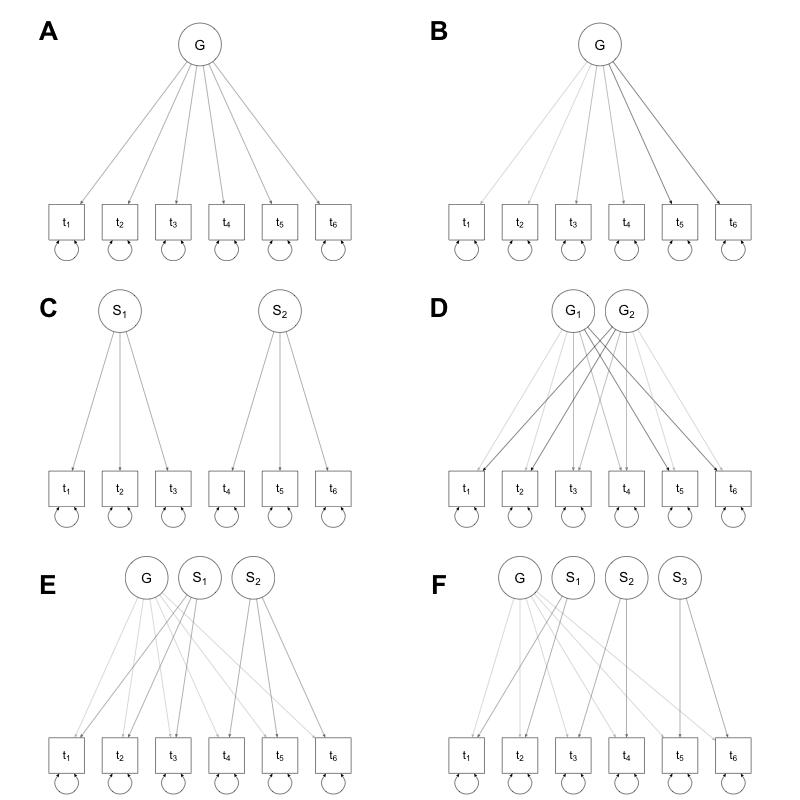
\includegraphics[width=\linewidth, height=1.1\linewidth, keepaspectratio]{_figs/factor_tree.png}
    \caption{TK}  % Replace 'TK' with your actual caption.
    \label{fig:fac_st}
\end{figure}


\end{document}